\section{Ejercicio 4}
\subsection{El Problema}

Se tiene un conjunto de etiquetas y una permutación de éstas. Es decir, para cada etiqueta $i$, se conoce $P(i)$. El problema consiste en, interpretando las etiquetas y sus permutaciones como dos conjuntos distintos de vértices de grafos, dar la cantidad de posibles grafos dirigidos completos que pueden construirse con esos vértices de forma tal que sean automorfos. Se pide implementar un algoritmo que resuelva este problema con complejidad del orden de $O(N^2*log(N))$

\subsection{Desarrollo}

Se particionan los elementos en ciclos de permutación. Es decir, ciclos de la forma $i => P(i) => P(P(i)) => ... => i$. Cada elemento pertenecerá a un único ciclo. Primero se demostrará que, si alguno de dichos ciclos posee longitud par, entonces la cantidad de grafos automorfos posibles será 0.

\subsubsection{Ciclos Pares}

Sean los elementos del ciclo $0..n-1$ con $n$ par. Supongamos, sin pérdida de generalidad, que en el grafo a armar hay un eje que va de $0$ a $n-1$ y que el ciclo tiene ejes de $i$ a $i+1$. Como hay un eje de $0$ a $n-1$, también va a tener que haber uno entre $P(0)$ y $P(n-1)$, que en este caso van a ser $1$ y $n$ (porque la permutación es un ciclo con ejes de $i$ a $i+1$). De esta forma, se obtiene que debe haber un eje de $n-1$ a $2n-1$ (recordar que en el problema esto significa un resultado. Es decir, $n-1$ le gana a $2n-1$. Pero el elemento $2n-1-esimo$ del ciclo es en realidad el $0$. Entonces $0$ le gana a $n-1$ y $n-1$ le gana a $0$. Entonces si hay un ciclo de permutacion de longitud par, la cantidad de grafos automorfos a armar será 0.

\subsubsection{Ciclos Impares}

Se quiere ver cuántos grafos automorfos posibles hay si la permutación consiste únicamente de un ciclo. Es decir, dados $n$ vértices, la permutación es un ciclo de $n$. Suponemos que en el ciclo de la permutación, hay un eje del elemento $i$ al $i+1$. Entonces lo que se quiere ver es cuántas decisiones hay que tomar a la hora de elegir los distintos posibles ejes del grafo completo. Supongamos que se tienen 7 vértices con la permutación dicha. Todos los elementos que están a distancia uno en la permutación, es decir, los pares $(i,i+1)$ deben tener algún eje en el grafo a armar. Entonces, sea 0 el primer elemento. Al decidir la dirección del eje entre 0 y 1, se ve que, por la permutación, quedan definidos todos los otros ejes de elementos a distancia uno. Esto es, como 0 le gana a 1, entonces $P(0)=1$ le tiene que ganar a $P(1)=2$ y así sucesivamente. Entonces, en el grafo de resultados que se va armando quedaría así.

\begin{figure}[H]\centering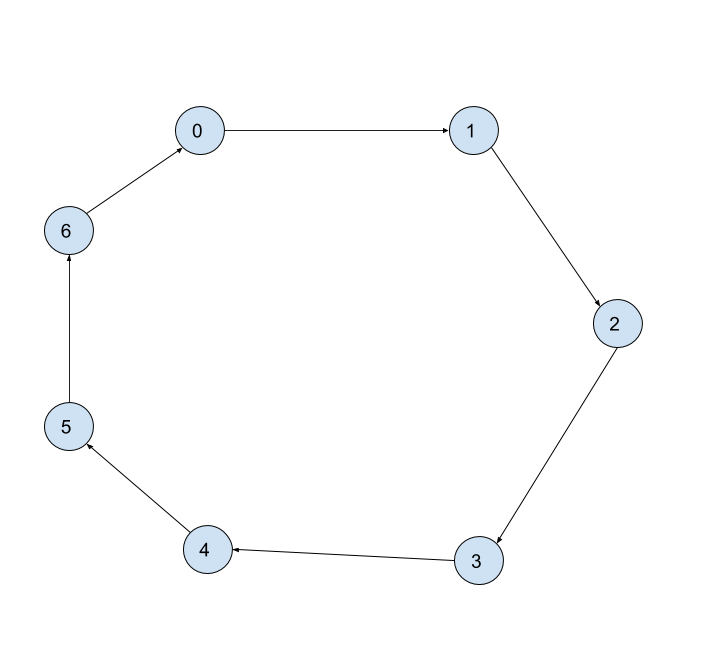
\includegraphics[scale=0.4]{Imagenes/Ej4a.png}\caption{Resultados de distancia 1}\end{figure}

Entonces, podemos ver que al definir uno de los resultados posibles de elementos a distancia 1, se definen los restantes. Entonces, hay solo una decisión por tomar. O $0$ le gana a $1$, o $1$ le gana a $0$. Para elegir los resultados de elementos a distancia dos, pasa algo similar. Supongamos que el $0$ le gana al $2$. Siguiendo un razonamiento similar, todos los resultados siguientes de elementos a distancia dos quedan definidos, de la siguiente manera.

\begin{figure}[H]\centering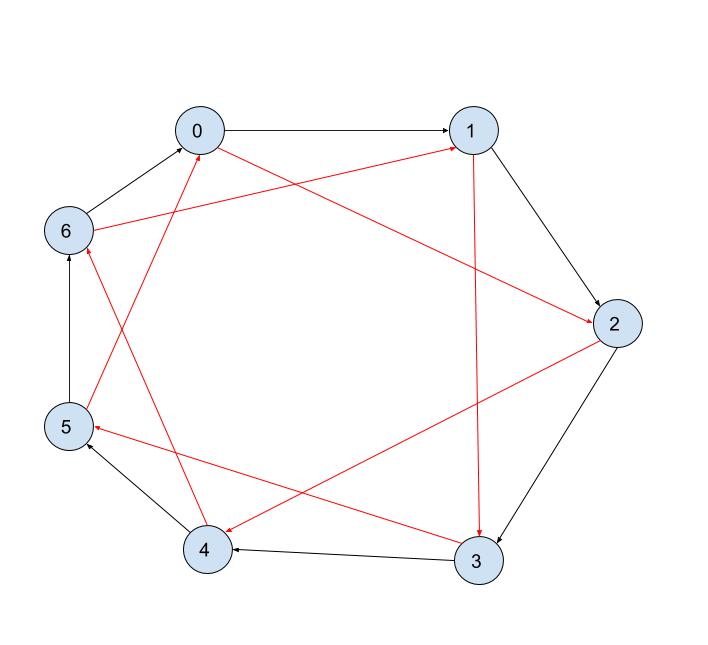
\includegraphics[scale=0.4]{Imagenes/Ej4b.png}\caption{Resultados de distancia 1 y 2}\end{figure}

Entonces aquí sólo se tomó una decisión más. Para elegir los posibles resultados de elementos a distancia dos, sólo hace falta decidir si $0$ le gana a $2$ o si $2$ le gana a $0$. Se procede a elegir los de longitud 3. Si se parte de que $0$ le gana a $3$, nuevamente quedan todos los resultados definidos, dándo lugar al siguiente grafo.

\begin{figure}[H]
\centering
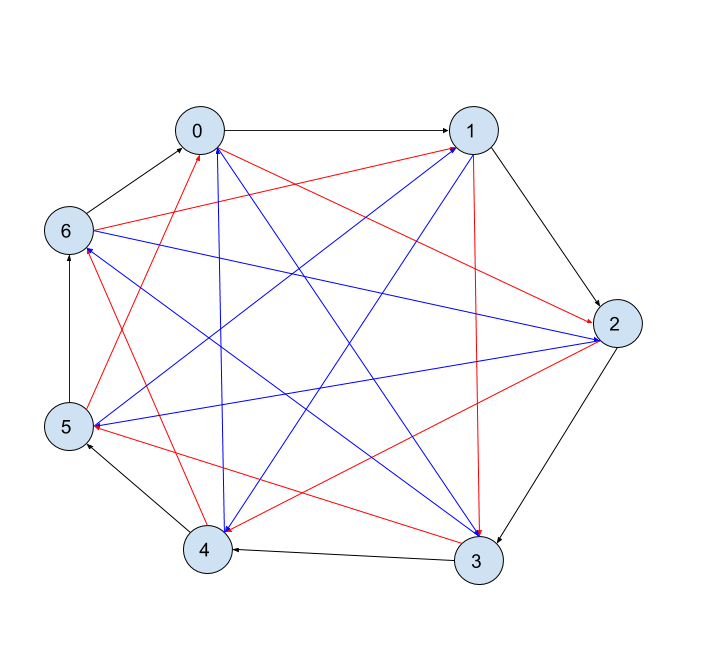
\includegraphics[scale=0.4]{Imagenes/Ej4c.png}
\caption{Resultados de distancia 1, 2 y 3}
\end{figure}

Nuevamente se tomó una única decisión. Si se observa, ya están todos los ejes del grafo. Esto es porque al agregar los ejes entre elementos a distancia 1, se agregaron los de elementos a distancia 6. Esto es, porque si bien $0$ está a distancia uno de $1$, $1$ está a distancia $6$ de 0. Entonces, se tomaron $\left \lfloor{n/2}\right \rfloor$ decisiones, y cada una de dichas decisiones tiene dos posibles opciones. Entonces, la cantidad de grafos posibles es $2^{\left \lfloor{n/2}\right \rfloor}$.

Por lo tanto, dado un ciclo de permutación de longitud impar, la cantidad de resultados posibles es $2^{\left \lfloor{n/2}\right \rfloor}$.

\subsubsection{Caso General}

Por último, falta ver lo que sucede cuando se tiene más de un ciclo en la permutación. Sean $A$ y $B$ dos ciclos de longitud impar. Supongamos que $A$ tiene longitud 3 y $B$ tiene longitud 5. Supongamos que los elementos de ambos son llamados $a_i$ y $b_j$ con $i \in \{0..2\}$ y $j \in \{0..4\}$. Supongamos también que las permutaciones son de la forma $P(i)=i+1$. La cantidad de ejes necesarios entre los elementos de $A$ y $B$ es $A*B$. Esto es, porque cada elemento de $A$ debe conectarse con cada elemento de $B$. La pregunta que resta formularse es cuántas decisiones hay que tomar.

Supongamos que $a_0$ le gana a $b_0$. Entonces, $P(a_0)$ debe ganarle a $P(b_0)$. Queremos ver cuántos ejes define esta decisión. El número de ejes que defina debe ser múltiplo de 3 (la longitud de $A$). Esto es porque, si definimos un eje para $a_0$, se van a definir ejes automáticamente para los elementos restantes de $A$. Pero también debe ser múltiplo de 5 (la longitud de $B$). Veamos por qué. En el ejemplo, una vez se llega a que $a_2$ debe ganarle a $b_2$, se sabe que $P(a_0)$ debe ganarle a $P(b_3)$. Este eje es nuevo, a pesar de que se vuelve a ver $a_0$. Para que se termine de ver la cantidad de ejes nuevos, es necesario volver a llegar a que $a_0$ le gana a $b_0$. Entonces la cantidad de ejes también va a ser múltiplo de la longitud de $B$. Por lo tanto, la cantidad de ejes definidos es el $MCM$ (Mínimo Común Múltiplo) de las longitudes de $A$ y $B$. Esto es porque recién ahí volvemos a ver $a_0$ y $b_0$.

Entonces, se tienen $A*B$ ejes y cada decisión tomada impacta $MCM(A,B)$ ejes. Por lo tanto, la cantidad de decisiones posibles es $\frac{A*B}{MCM(A,B)}$.

Supongamos que $A=X*T$ y $B=Y*T$, con $X$ e $Y$ coprimos. El $MCM(A,B)$ es igual a $X*Y*T$. Entonces si se reemplaza en la cuenta, se obtiene que la cantidad de decisiones es $T$, dónde $T$ es el $MCD(A,B)$. Entonces, como cada decisión tiene dos opciones posibles, entre dos ciclos de longitud impar de longitudes $A$ y $B$, la cantidad de resultados posibles entre ambos es $2^{MCD(A,B)}$.

Por lo tanto, dada una permutación, primero se divide en ciclos. Si algún ciclo es par, entonces la cantidad de resultados posibles es 0. Si todos son impares, se multiplica la cantidad de resultados de cada ciclo por separado y luego por cada par de ciclos distintos. Ese es el resultado buscado.

\subsubsection{Implementación}

Se presenta a continuación un pseudocódigo del ejercicio.

\begin{verbatim}
inicializar()
armarCiclos()
if(hayCiclosPares()) return 0
else return calcularResultadosPosibles()
\end{verbatim}

La función \texttt{inicializar()} lee la entrada, guardando la permutación, e inicializa vectores donde se guardarán las longitudes de los distintos ciclos y el ciclo al que pertenece cada elemento.

La función \texttt{armarCiclos()} calcula la longitud del ciclo al que pertenece cada elemento. Cuando visita un nuevo elemento, si éste ya se marcó como perteneciente a algún ciclo, lo saltea. Si no, comienza a recorrer el ciclo y va guardando la longitud del mismo, marcando los elementos que recorra.

La función \texttt{hayCiclosPares()} se fija si hay algún ciclo de longitud par.

La función \texttt{calcularResultadosPosibles()} realiza la cuenta correspondiente. Primero itera sobre los ciclos y va multiplicando la cantidad de resultados posibles para cada uno y luego itera sobre los pares y hace lo mismo para cada par.
Para hacer esto se debe calcular el MCD. Esto se hace con el algoritmo visto en clase. Además, para elevar 2 a los números correspondientes, se implementó una función \texttt{modexp} que usa el algoritmo visto en clase para calcular potencias haciendo el módulo con $10^9 + 7$ en cada paso para evitar overflow.

\subsubsection{Complejidad}

Se analizará a continuación la complejidad del algoritmo.

La complejidad de la función \texttt{inicializar()} es de \O{N}. Esto es porque lee la entrada, e inicializa una cantidad constante de vectores de tamaño $N$.

La complejidad de la función \texttt{armarCiclos()} es de \O{N}. Esto es porque recorre todos los elementos a lo sumo dos veces. Recorre todos una vez. Si ya pertenecen a un ciclo, recorre el ciclo. Si no, no. Como cada elemento pertenece a un único ciclo, en el peor caso recorre todos los elementos una vez y todos los elementos otra vez para ver los ciclos.

La complejidad de la función \texttt{hayCiclosPares()} es de \O{N}. Esto es porque recorre el vector de longitudes de ciclos y se fija si hay alguno par. A lo sumo hay $N$ ciclos.

La función \texttt{calcularResultadosPosibles()} consiste de dos ciclos. En el primero se itera sobre todos los ciclos de la permutación (a lo sumo $N$) y se realiza una cuenta involucrando la función \texttt{modexp()}. La complejidad de \texttt{modexp()} (vista en clase) es logarítmica en el exponente y el exponente siempre es menor o igual a $N$. Por lo tanto la complejidad de este ciclo es \O{N*log(N)}.

En el segundo ciclo, itera sobre todos los pares de ciclos (son \O{N^2} pares) y por cada uno calcula el $MCD$ entre sus longitudes. El algoritmo de $MCD$ es el visto en clase, de complejidad logarítmica en el máximo de las longitudes de ambos (ambas acotadas por $N$ porque se trata de ciclos en la permutación).
Luego, calcula $2^{MCD}$ utilizando la función \texttt{modexp()}. Esto es de complejidad logarítmica en $MCD$ (éste está acotado por el máximo de ambos, que a su vez está acotado por $N$). Entonces, por cada par de ciclos (\O{N^2}) se realizan dos operaciones de \O{log(N)}.

Entonces, la función es de complejidad \O{N*log(N) + N^2*log(N)}. Esto es \O{N^2*log(N)}.

Por lo tanto, la complejidad del algoritmo es de \O{N + N + N + N^2*log(N)}. Esto es \O{N^2*log(N)}.

\subsection{Puntaje}
El peso otorgado a este ejercicio es: 9
